
In order to sail properly and make the most out of the wind that’s is supplied by the nature itself some data acquisition is needed. The sailing is all about this harnessing all the forces of the nature and the wind that it pushing towards you. Since there has not been any other extensive projects and measurements in this particular area the measurements have to be done in new ways. 

\subsection{Force sensors}

The goal here is to have a system that can measure the forces that pushes on the centerboard by the water it goes through. 
The implementation:
By looking at some different solutions there is not any other solutions that might be as clean looking and prominent as this approach. Important to know is that every solution is mandatory to be waterproof and sealed properly from the harsh environment that this system has as its home turf. The solutions that required the sensors to be mounted on the outside or in parts that would be in danger if a crash might occur was scratched.  
The board itself will not be disassembled in any major part of way. Meaning that this approach doesn’t need any modifications to the board itself. This has been the goal and the choosen approach. Modifications in the mounting plate is the way to go, the other solutions is either way more difficult to apply and mount or more complex.

\subsection{The prototype}
To implement the gauges, a prototype is designed to show how the measurements will be made. The prototype is a bit bigger than the intended solution for this project but it's good to see how it would be constructed. The function is easy to understand. The board goes on the outside and can easily slide up and down past this ball.  The ball itself is kept inside this small area where it can move in and out.
 
\begin{figure}[H]
\begin{center}
	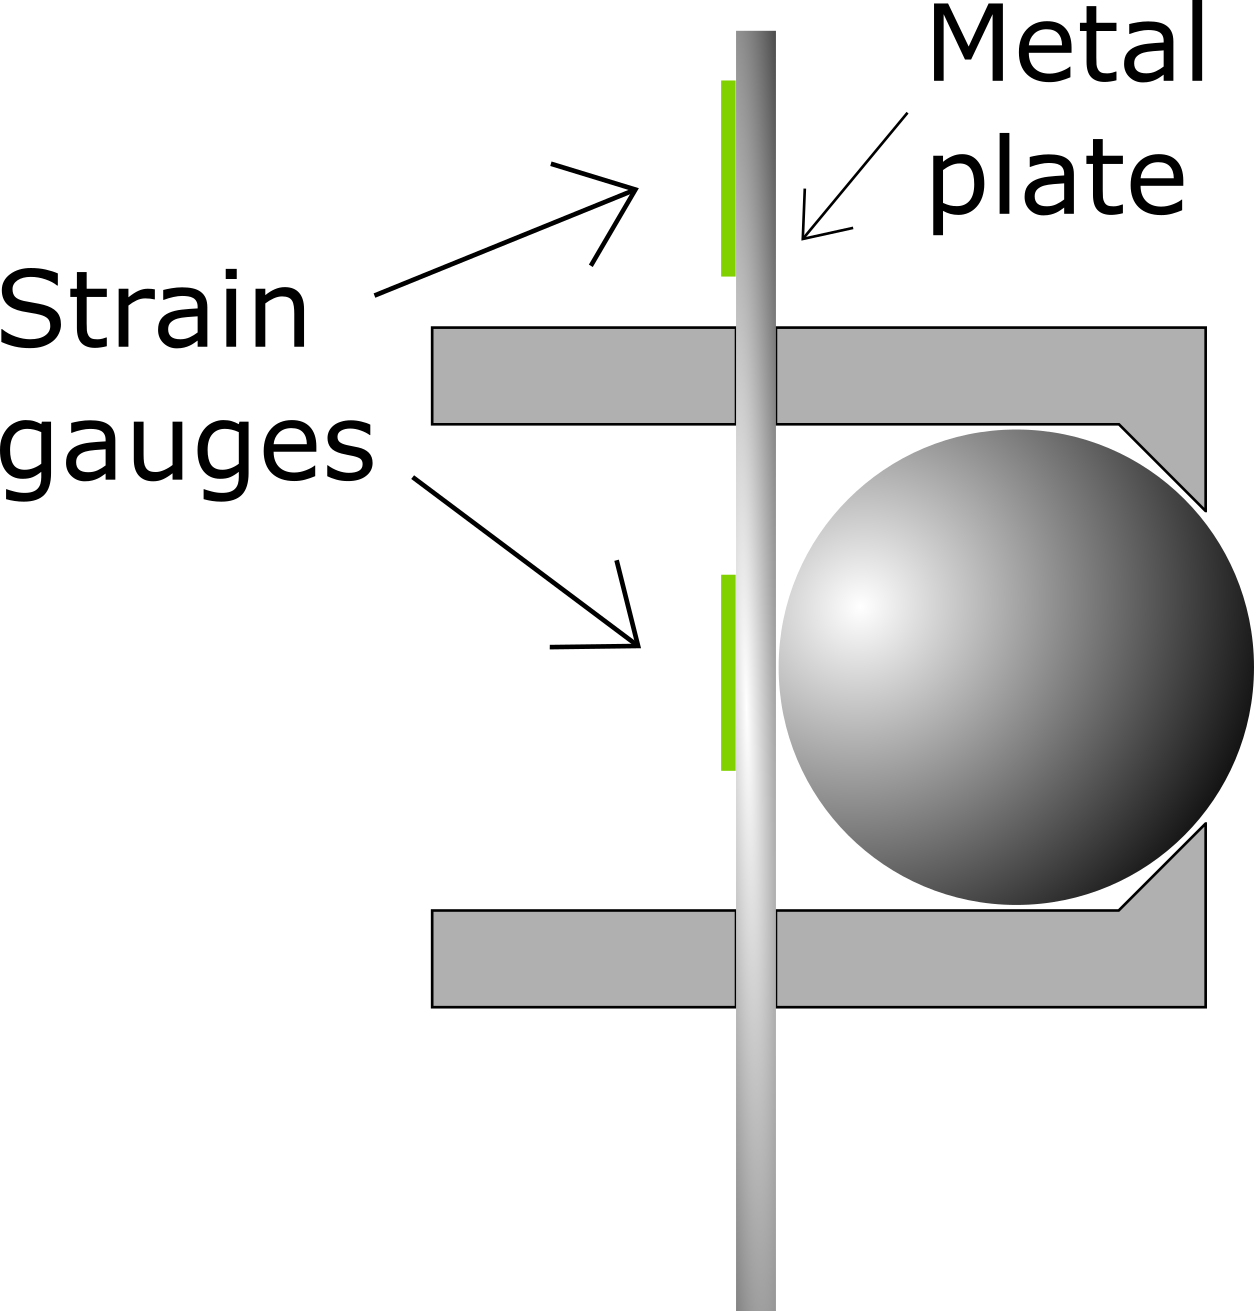
\includegraphics[width = 10cm]{Figures/Press_sens_func_1.png}
	\caption{Function of first prototype}
	\label{Press_sens_prot_1}
\end{center}
\end{figure}

This way of implementing strain gauges was the first idea. 
The main case for this strategy was that in the start of this project these gauges were supplied to us, as a leftover from the last group. With this implementation, we could already start working on a prototype and get a small head start in to the project. But as some research shows, it is a more difficult way to solve this problem and it would take bit more work and some sensitive circuits to measure the force. The gauges also need to be stuck in place using some specific glue and can easily be done incorrectly and therefore prevent good measurements.

A model of the pressure sensor was constructed in the CAD program fusion 3D. This model was created in order to clearly show the function of this sensor and to help the thought process involved in the improving of this design.

\begin{figure}[H]
\begin{center}
	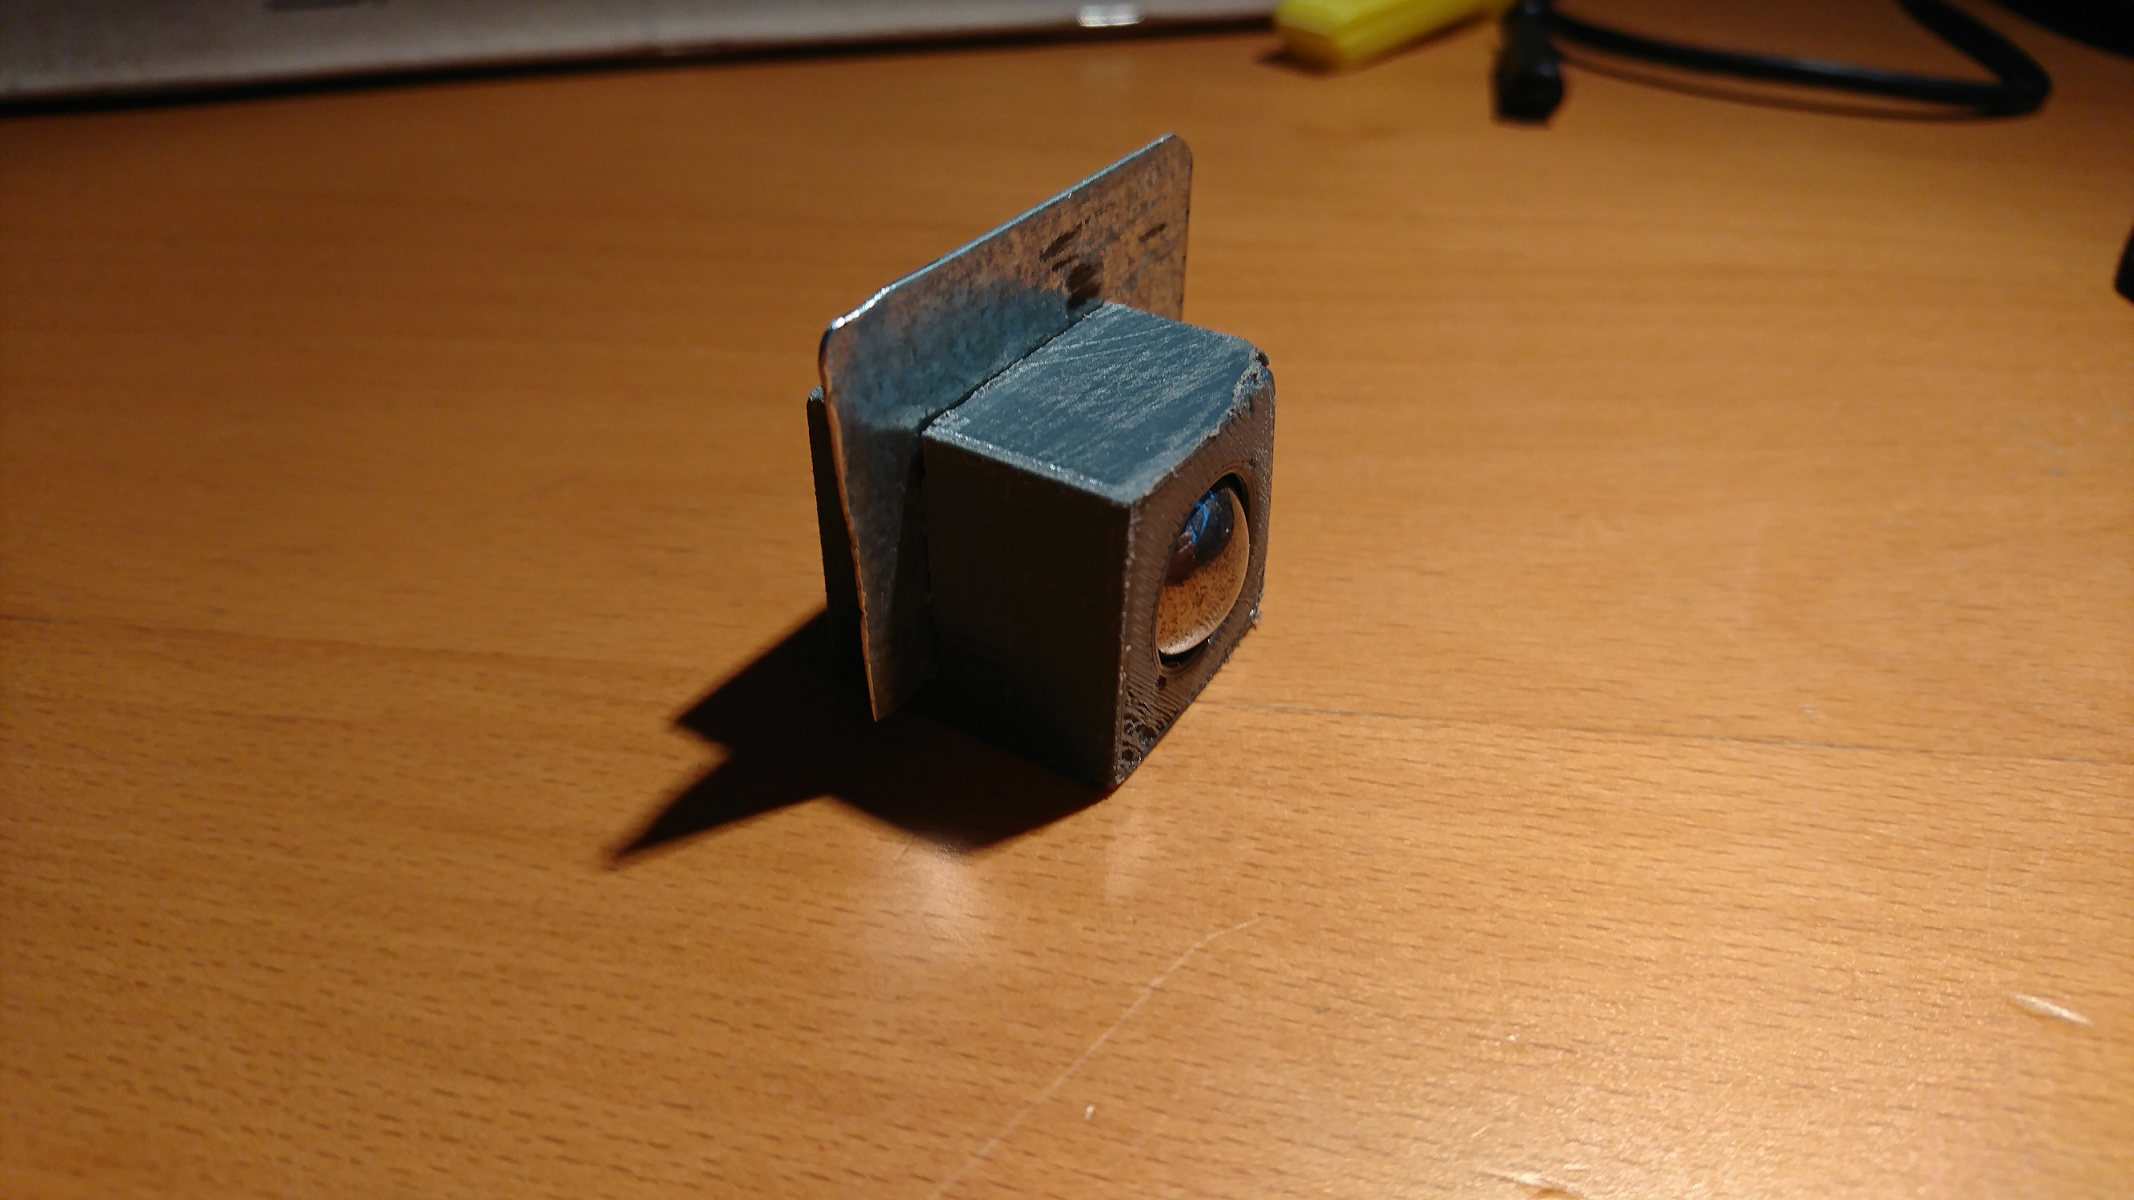
\includegraphics[width = 10cm]{Figures/Press_sens_prot_1.png}
	\caption{Function of first prototype}
	\label{Press_sens_prot_1}
\end{center}
\end{figure}
 The force is then measured at the back where there will be a plate. The deflection of this plate which will be the origin to the strain will be measured through strain gauges. 
The gauge itself will measure a small difference in resistance. This small difference is going to be difficult to measure without any amplifying circuit connected. With a such small signal the system might have issues with noise. Another problem is the signal might drift, and therefore make different measurements as the circuit is running. And finally, with the measured values getting amplified with a big amount the resulting signal may be off by a large amount. 

New idea:
A better solution is to make some research into load cells, which is a sensor which also utilizes strain gauges to measuring forces. The difference is that the gauges are already implemented in the sensor. The difference in the prototype is instead of having a metal plate, it can be built with a piece of plastic or rubber which can deform so the force is distributed directly to the sensor. By implementing this sensor, a lot of time was saved in troubleshooting. And by having a sensor unit, the modified mounting plate will be easier to produce. 
 
\begin{figure}[H]
\begin{center}
	
\includegraphics[width = 10cm]{Figures/Press_sens_func_2.png}
	\caption{Function of second prototype}
	\label{Press_sens_prot_2}
\end{center}
\end{figure}

\subsection{Choice of component}

The force from the board onto the mounting plate will be a considerable amount. The actual force is something that’s not known for sure. The initial assumption was that a load cell with a 90.75 kg force range should be enough. In the case the sensor will be maxed out the cell it's rated for a 150\% overload without causing some damage to the sensor.
The choosen sensor for this application is selected to this part, the compression load cell called FX1901. 
From the datasheet the voltage readings of this piece could be calculated. With a maximum voltage reading of around $36mV/V$

 \begin{figure}[H]
\begin{center}
	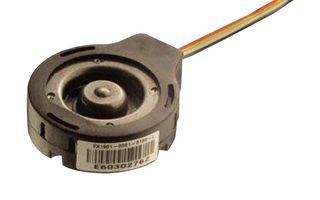
\includegraphics[width = 10cm]{Figures/Load_cell.png}
	\caption{Load cell, FX1901}
	\label{Load_cell}
\end{center}
\end{figure}



\subsection{Amplifier}


In order for the microcontroller to make some good measurements from the load cell an amplification for the  
That’s a small signal and needs to be amplified to get some good measurements. A good measurement signal to the MCU should be in the order of in between 0 - 5 volts. 
This is achieved by an amplification gain of around 20. 


A suitable amplifier needs to be choosen from the vast ocean of different models. Inspiration is taken from The university of Chicago\ref{UoC} in an experiment where they uses this exact load cell togheter with an instrumental amplifier called INA125. This amplifier is somewhat more complicated and have some more feautures that other amplifiers. In the same family of instrument amplifiers a model called INA126 is selectet as a less complicated and more power efficiant solution.


The choice fell on this little fellow, the INA126. 

\begin{figure}[H]
\begin{center}
	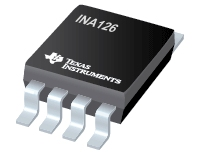
\includegraphics[width = 10cm]{Figures/INA126.png}
	\caption{Amplifier for the load cell signal}
	\label{INA126}
\end{center}
\end{figure}


Which not look so interesting but has the benefit of having a smaller power consumption then many others by being a bit simpler than many others. But sufficient for our purpose.

It seems like a smart choice because when the system is battery operated, like in this case, every watt counts.
The gain on this piece is easily calculated with this function. Gain is 5 plus 80k ohm divided by our chosen resistor Rg.

 \begin{figure}[H]
\begin{center}
	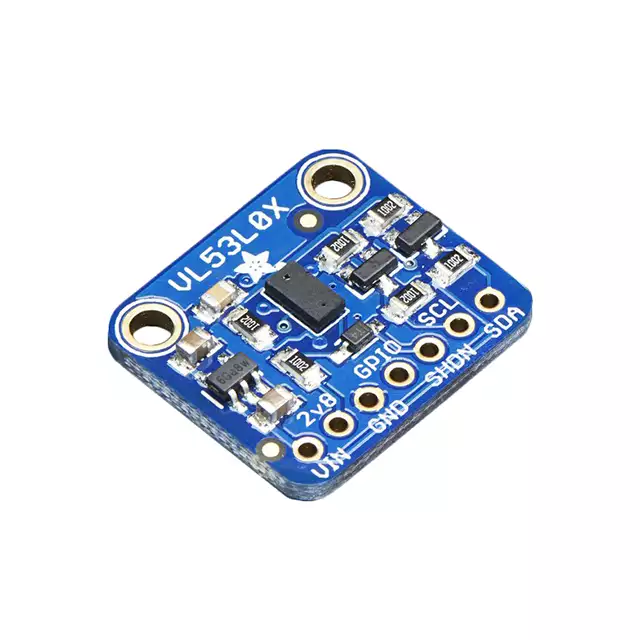
\includegraphics[width = 10cm]{Figures/Adafruit_height_sensor.png}
	\caption{Time of flight distance sensor, Adafruit VL53L0X}
	\label{micro_lidar}
\end{center}
\end{figure}

If our desired 20 gain might not work or the voltages calculated is off, the gain is easily redone with this expression.
\begin{equation}
Gain = 5 + \frac{80k\Omega}{R_G}
\end{equation}


Now that we know how to get the force measurements, we are going to talk about how to measure the frequency of waves at sea.


\subsection{Height of daggerboard sensor}

The main issues might be that the Height of daggerboard: 
One of the best implementations of a height sensor would be the use of a linear wire distance sensor. This particular sensor measures how far a wire is pulled, which gives a very accurate measurement. This solution can be totally watertight and concealed in the main centerplate.  

 \begin{figure}[H]
\begin{center}
	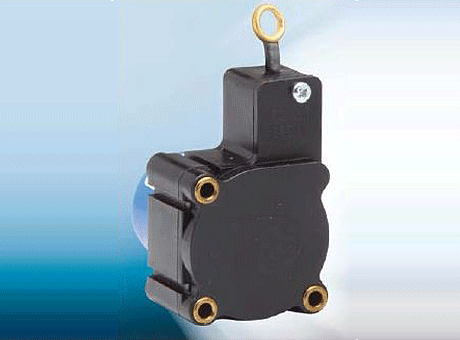
\includegraphics[width = 10cm]{Figures/microepsilon_mk30.png}
	\caption{Linear draw wire sensor, Micro epsilon MK30}
	\label{Draw_sensor}
\end{center}
\end{figure}
 
We have found some sensors that might work for us, this is the smallest we found. It's 3 cm wide and about 5 cm high. As we have some tight space constraints this can probably fit inside or just stick out a little bit. This particular sensor is in the range of 2000 kr, which feel like a lot. But if no other solution works this might be considered again.  


We have also looked into some light sensors. This is implemented with the use of a plate placed ion top of the dagger-board and with the light being sent up to this panel, the height can be calculated. First we looked into some ir-sensors. They will probably send the signal in a wide spread which will make the distance measurement troublesome as this signal has just a small plate to bounce of.  
  

But with the use of a LIDAR system, we can point our light signal at an exact spot and then get an exact measurement of the height.  
Many of the lidar systems we found was too big for our project and also very expensive.  
A suitable sensor that we found was a small "micro lidar" circuit from adafruit: 




\subsubsection{Component}



 \begin{figure}[H]
\begin{center}
	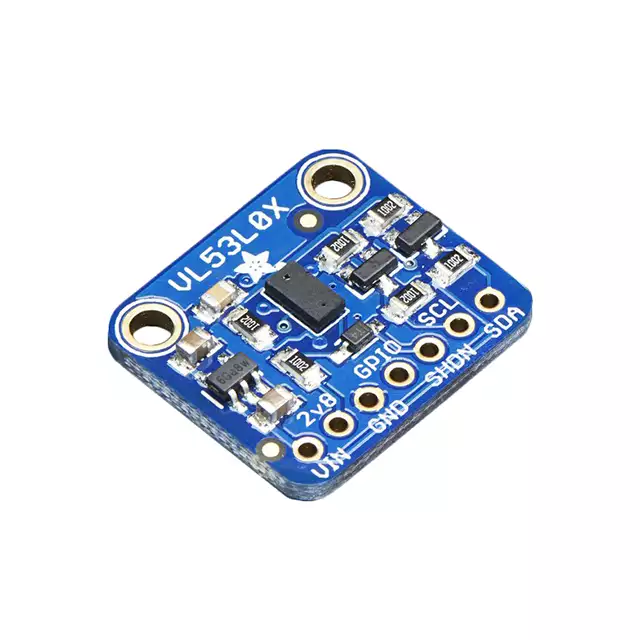
\includegraphics[width = 10cm]{Figures/Adafruit_height_sensor.png}
	\caption{Time of flight distance sensor, Adafruit VL53L0X}
	\label{micro_lidar}
\end{center}
\end{figure}
Problems: 

As there will always be water around and on the centerplate the light that is sent might get directed "wrong" if there is only some small water droplets in between the sensor and the panel that we want to reflect our light on. 

By the fact that the senor have to be water proof the signal has to go through a medium. The medium can be some type of plastic or even glass.  
If the signal can be read correctly through this medium or if the signal will get corrupted, we don't know yet. That is something that we need to test later when our parts has come in. 



